% !TEX root = main2.tex
\section{Modeling/semantic framework}
\label{sec:prelims}

%We assume that the discrete states or the modes and their transition rules are  known, but  the  dynamic models for the continuous state variables are not. Instead, we can only use sampled data of continuous trajectories, obtained by, for example, simulations or tests. 
We introduce a powertrain control system from~\cite{jin2014powertrain}
as a running example to illustrate the elements of our hybrid system
modeling framework.

\subsection{Powertrain  control system}
\label{ex:powertrain}

This system ($\auto{Powertrn}$) models a highly nonlinear engine control system. The relevant state variables of the model are intake manifold pressure ($p$), air-fuel ratio ($\lambda$), estimated manifold pressure ($pe$) and intergrator state ($i$).
The overall system can be in one of four modes
$\Lmode{startup}$,
$\Lmode{normal}$,
$\Lmode{powerup}$, 
$\Lmode{sensorfail}$. 
A \Simulink\ diagram describes the continuous evolution of the above variables. 
%\mitras{Disambiguate which version of the model we are using and say something about Simulink model.} 
In this paper, we mainly work on the {\em Hybrid I/O Automaton Model}
in the suite of powertrain control models. The \Simulink\ model
consists of continuous variables describing the dynamics of the
powertrain plant and sample-and-hold variables as the controller.  One
of the key requirements to verify is that the engine maintains the
air-fuel ratio within a desired range in different modes for a given
set of driver behaviors. This requirement has implications on fuel
economy and emissions.
%
For testing purposes, the control system designers work with sets of driver profiles that essentially define families of switching signals across the different modes. 
Previous verification results on this problem have been reported in~\cite{DFMV:CAV2015, FDMV:ARCH2015} on a simplified version of the powertrain control model.

\vspace{-10pt}
\subsection{Transition graphs}
\label{ssec:modes}
We will use  $\L$ to denote a finite set of {\em modes\/} or locations of the system under consideration. The discrete behavior or mode transitions are specified by what we call a transition graph over $\L$.
\begin{definition}
	 A {\em transition graph\/} is a labeled, directed acyclic
         graph $G = \langle \L, \V, \E, \vertlab, \edgelab \rangle$,
         where
	\begin{inparaenum}[(a)]
	\item $\L$ is the set of vertex labels also called the set of
          {\em modes\/},
	\item $\V$ the set of vertices, 
	\item $\E\subseteq \V \times \V$ is the set of edges, 
	\item $\vertlab: \V \rightarrow \L$ is a vertex labeling
          function that labels each vertex with a mode, and
	\item $\edgelab: \E\rightarrow \nnreals \times \nnreals$ is an
          edge labeling function that labels each edge with a
          nonempty, closed, bounded interval defined by pair of
          non-negative reals.
	\end{inparaenum}
\end{definition}
Since $G$ is a DAG, there is a nonempty subset $\V_{\sf init}
\subseteq \V$ of vertices with no incoming edges and a nonempty subset
$\V_{\sf term} \subseteq \V$ of vertices with no outgoing edges.  We
define the set of initial locations of $G$ as $\L_{\sf init} = \{ \ell
\ | \ \exists \ v \in \V_{\sf init}, \vertlab(v) = \ell \}$.
% 
A (maximal) {\em path\/} of the graph $G$ is a sequence $\pi = v_1,
t_1, v_2, t_2, \ldots, v_k$ such that,
\begin{inparaenum}[(a)]
\item $v_1 \in \V_{\sf init}$,
\item $v_k \in \V_{\sf term}$, and 
\item for each $(v_i,t_i,v_{i+1})$ subsequence, there exists $(v_i, v_{i+1}) \in \E$, and $t_i \in \edgelab((v_i,v_{i+1}))$.
% 
\end{inparaenum}
%
$\paths{G}$ is the set of all possible paths of $G$.  For a given path
$\pi = v_1, t_1, v_2, t_2, \ldots,$ $v_k$ its {\em trace\/}, denoted by
$\vertlab(\pi)$, is the sequence $\vertlab(v_1), t_1, \vertlab(v_2),
t_2, \ldots,$ $\vertlab(v_k)$.  Since $G$ is a DAG, a trace of $G$ can
visit the same mode finitely many times.  $\traces{G}$ is the set of
all traces of $G$.
%
% comment about finite unrollings.
%
%

An example transition graph for the $\auto{Powertrain}$ system of Section~\ref{ex:powertrain} is shown in Figure~\ref{fig:power_graph}. The set of vertices $\V = \{0,\ldots, 4\}$ and the $\vertlab$'s and $\edgelab$'s appear adjacent to the vertices and edges. 
%
\begin{figure}[h]
	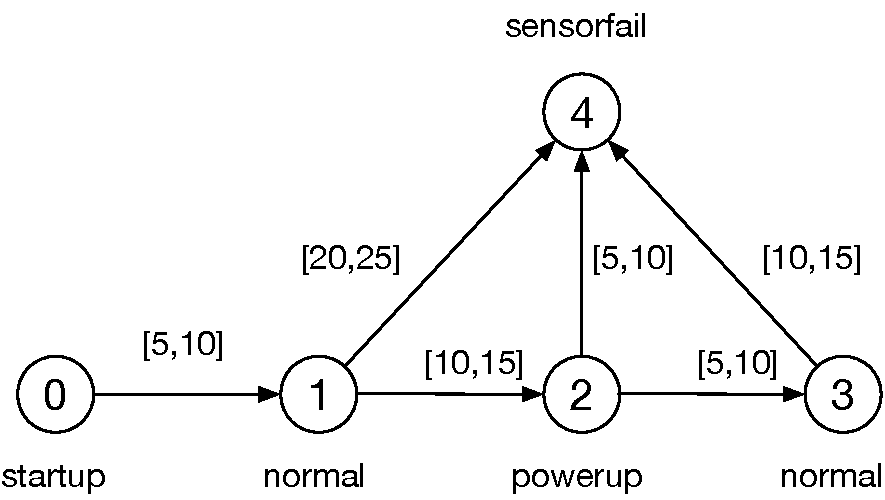
\includegraphics[scale=0.4]{power_graph1.pdf}
	\vspace{-10pt}
	\caption{\small A sample transition graph for $\auto{Powertrain}$ system.}
	\label{fig:power_graph}	
\end{figure}
\vspace{-8pt}
\subsubsection{Trace containment}
We will develop reasoning techniques based on reachability,
abstraction, composition, and substitutivity. To this end, we will
need to establish containment relations between the behaviors of
systems. Here we define containment of transition graph traces.
Consider transition graphs $G_1, G_2,$ with modes $\L_1,\L_2,$ and a
mode map $\modemap: \L_1 \rightarrow \L_2$.  For a trace $\sigma =
\ell_1, t_1, \ell_2, t_2, \ldots, \ell_k \in \traces{G_1}$,
simplifying notation, we denote by $\modemap(\sigma)$ the sequence
$\modemap(\ell_1), t_1, \modemap(\ell_2), t_2,$ $\ldots,
\modemap(\ell_k)$.  We write $G_1 \preceq_{\modemap} G_2$ iff for
every trace $\sigma \in \traces{G_1}$, there is a trace $\sigma' \in
\traces{G_2}$ such that $\modemap(\sigma)$ is a prefix of $\sigma'$.
%


\begin{definition}
Given graphs $G_1, G_2$ and a mode map $\modemap: \L_1 \rightarrow
\L_2$, a relation $R \subseteq \V_1 \times \V_2$ is a {\em forward
  simulation relation from $G_1$ to $G_2$\/} iff
\begin{enumerate}[(a)]
\itemsep0em 
	\item for each $v \in \V_{1 {\sf init}}$, there is $u \in
          \V_{2 {\sf init}}$ such that $(v,u) \in R$,
        \item for every $(v,u) \in R$,  $\modemap(\vertlab_1(v)) =
          \vertlab_2(u)$, and
	\item for every $(v,v') \in \E_1$ and $(v,u)\in R$, there
          exists a finite set $u_1, \ldots, u_k$ such that:
	\begin{inparaenum}[(i)]
		\item for each $u_j$, $(v,u_j) \in R$, and
		\item $\edgelab_1((v,v')) \subseteq \cup_j
                  \edgelab_2((u,u_j))$.
	\end{inparaenum}
\end{enumerate}
\end{definition}

\begin{proposition}
	\label{prop:graphsim}
	If there exists a forward simulation relation from $G_1$ to
        $G_2$ with $\modemap$ then $G_1 \preceq_{\modemap} G_2$.
\end{proposition}
%For this to make sense, $G$ must have some (boring) well-formedness properties like the $\edgelab(e)$ should be nonempty for each $e$.

%\mitras{Statement about complexity of checking $G_1 \preceq G_2$.}
%$\Sigma(G)$ = union over all paths. 
\vspace{-10pt}
\subsubsection{Sequential composition of graphs}

We will find it convenient to define the \emph{sequential composition}
of two transition graphs. Intuitively, the traces of the composition
of $G_1$ and $G_2$ will be those that can be obtained by concatenating
a trace of $G_1$ with a trace of $G_2$. To keep the definitions and
notations simple, we will assume (when taking sequential compositions)
$|\V_{\sf init}| = |\V_{\sf term}| = 1$; this is true of the examples
we analyze. It is easy to generalize to the case when this does not
hold. Under this assumption, the unique vertex in $\V_{\sf init}$ will
be denoted as $v_{\sf init}$ and the unique vertex in $\V_{\sf term}$
will be denoted as $v_{\sf term}$.

\begin{definition}
\label{def:seq-comp}
Given graphs $G_1 = \langle \L, \V_1, \E_1, \vertlab_1, \edgelab_1
\rangle$ and $G_2 = \langle \L, \V_2, \E_2,$ $\vertlab_2, \edgelab_2
\rangle$ such that $\vertlab_1(v_{1 {\sf term}}) = \vertlab_2(v_{2
  {\sf init}})$, the \emph{sequential composition} of $G_1$ and $G_2$
is the graph $G_1\seqcomp G_2 = \langle \L, \V, \E, \vertlab, \edgelab
\rangle$ where
\begin{enumerate}[(a)]
\itemsep0em 
\item $\V = (\V_1 \cup \V_2) \setminus \{v_{2 {\sf init}})\}$,
\item $\E = \E_1 \cup \{(v_{1 {\sf term}},u)\: |\: (v_{2 {\sf
    init}},u) \in \E_2\} \cup \{(v,u) \in \E_2\: |\: v \neq v_{2 {\sf
    init}}\}$,
\item $\vertlab(v) = \vertlab_1(v)$ if $v \in \V_1$ and $\vertlab(v) =
  \vertlab_2(v)$ if $v \in \V_2$,
\item For edge $(v,u) \in \E$, 
$\edgelab((v,u)) $ equals \begin{inparaenum}[(i)]
                   \item $\edgelab_1((v,u))$, if $u \in \V_1$, \\
                   \item $\edgelab_2((v_{2 {\sf init}},u))$,  if $v = v_{1 {\sf term}}$,
                   \item $\edgelab_2((v,u)), otherwise$.
                          \end{inparaenum}
%$
%\edgelab((v,u)) = \left\{ \begin{array}{ll}
%                   \edgelab_1((v,u)) & \mbox{if } u \in \V_1\\
%                   \edgelab_2((v_{2 {\sf init}},u)) & \mbox{if } v = v_{1 {\sf term}}\\
%                   \edgelab_2((v,u)) & \mbox{otherwise}
%                          \end{array} \right.
%$
\end{enumerate}
\end{definition}

Given our definition of trace containment between graphs, we can prove
a very simple property about sequential composition.

\begin{proposition}
\label{prop:seqcomp-containment}
Let $G_1$ and $G_2$ be two graphs with modes $\L$ that can be
sequential composed. Then $G_1 \preceq_{{\sf id}} G_1\seqcomp G_2$,
where ${\sf id}$ is the identity map on $\L$.
\end{proposition}

The proposition follows from the fact that every path of $G_1$ is a
prefix of a path of $G_1\seqcomp G_2$. Later in Section \ref{sec: sub_exp} we see examples of sequential composition.

%mention powertrain example

%We assume that only the following are known:
%(a) a finite set $\L$ of possible discrete states or modes or locations,  
%(b) a set $\Sigma$ of switching signals or trajectories of $\L$ defining the time-evolution of the discrete state, 
%(c) a set $\Theta$ of initial states of the continuous variables,  
%(d) a set $\U$ of unsafe states.
%

\subsection{Trajectories}

The evolution of the system's continuous state variables is formally
described by continuous functions of time called {\em trajectories\/}.
Let $n$ be the number of continuous variables in the underlying hybrid
model. A {\em trajectory\/} for an $n$-dimensional system is a
continuous function of the form $\tau: [0,T] \rightarrow \reals^n$,
where $T \geq 0$. The interval $[0,T]$ is called the {\em domain\/} of
$\tau$ and is denoted by $\tau.\dom$. The first state $\tau(0)$ is
denoted by $\tau.\fstate$, last state $\tau.\lstate = \tau(T)$ and
$\tau.\ltime = T$.
%
For a hybrid system with $\L$ modes, each trajectory is labeled by a
mode in $\L$.  A {\em trajectory labeled by $\L$\/} is a pair $\langle
\tau, \ell \rangle$ where $\tau$ is a trajectory and $\ell \in \L$.
 
% assuming continuous in both first and second arguments.
% may need additional assumptions.
%For a given initial state $x_0 \in \reals^n$, $\tau(x_0,t)$ is the continuous state of the system following trajectory $\tau$ at time $t \in \tau.\dom$.
A {\em $T_1$-prefix\/} of $\langle \tau, \ell\rangle$, for any $T_1
\in \tau.\dom$, is the labeled-trajectory $\langle \tau_1,
\ell\rangle$ with $\tau_1:[0,T_1] \rightarrow \reals^n$, such that for
all $t \in [0, T_1]$, $\tau_1(t) = \tau(t)$.
%
A set of labeled-trajectories $\TL$ is prefix-closed if for any
$\langle \tau,\ell \rangle \in \TL$, any of its prefixes are also in
$\TL$.  A set $\TL$ is {\em deterministic\/} if for any pair $\langle
\tau_1, \ell_1 \rangle, \langle \tau_2,\ell_2 \rangle \in \TL$, if
$\tau_1.\fstate = \tau_2.\fstate$ and $\ell_1 = \ell_2$ then one is a
prefix of the other.
%
A deterministic, prefix-closed set of labeled trajectories $\TL$
describes the behavior of the continuous variables in modes $\L$.
%
We denote by $\TL_{\sf init,\ell}$ $=\{ \tau.\fstate \ | \ \langle
\tau,\ell \rangle \in \TL \}$, the set of initial states of
trajectories in mode $\ell$. Without loss generality we assume that
$\TL_{{\sf init},\ell}$ is a connected, compact subset of $\reals^n$.
%
We assume that trajectories are defined for unbounded time, that is,
for each $\ell \in \L, T >0$, and $x \in \TL_{{\sf init},\ell}$, there
exists a $\langle \tau, \ell \rangle \in \TL$, with $\tau.\fstate = x$
and $\tau.\ltime = T$.  
%\mitras{Probably need other
%  assumptions. Continuity, forward completeness.}


%
In control theory and hybrid systems literature, the trajectories are
assumed to be generated from models like ordinary differential
equations (ODEs) and differential algebraic equations (DAEs). Here,
we avoid an over-reliance on the models generating trajectories and
closed-form expressions. Instead, {\toolname} works with sampled data
of $\tau(\cdot)$ generated from simulations or tests.
	
\begin{definition}
	\label{def:sims}
A {\em simulator\/} for a (deterministic and prefix-closed) set $\TL$
of trajectories labeled by $\L$ is a function (or a program)
$\simulator$ that takes as input a mode label $\ell \in \L$, an
initial state $x_0 \in \TL_{\sf init,\ell}$, and a finite
sequence of time points $t_1, \ldots, t_k$, and returns a sequence of
states $\simulator(x_0,\ell,t_1), \ldots, \simulator(x_0,\ell, t_k)$
such that there exists $\langle\tau,\ell\rangle \in \TL$ with
$\tau.\fstate = x_0$ and for each $i\in \{1,\ldots, k\}$,
$\simulator(x_0,\ell,t_i) = \tau(t_i)$.
\end{definition}

The trajectories of the $\auto{Powertrn}$ system are described by a \Simulink\ diagram.
%
The diagram has several switch blocks and input signals  that can be set appropriately to generate simulation data using the \Simulink\ ODE solver.

%
For simplicity, we assume that the simulations are perfect (as in the
last equality of Definition~\ref{def:sims}). Formal guarantees of
soundness of {\toolname} are not compromised if we use \emph{validated
  simulations} instead.
% \mitras{In
%  Section~\ref{sec:verfication_algorithm}, we will see that the
%  soundness and relative completeness of the \toolname\ verification
%  algorithm is not compromised if we use validated simulation
%  instead. }
	
%which may be  difficult to implement in a computer program. Real numbers have to be approximately represented by a finite number of bits, numerical integrators approximate solutions of ODEs upto a certain precision, certain modes may not be well-defined in certain states or beyond certain times. We will ignore all of this in the current paper.


%For each discrete mode $\ell \in \L$, collection of deterministic prefix-closed set of trajectories $\{\T_\ell\}_{\ell \in \L}$.

%Continuity properties.

\vspace{-10pt}
\paragraph{Trajectory containment}
%We define containment of labeled trajectories.
%\mitras{In this paper we do not consider variable maps (only mode maps).} 
Consider sets of trajectories, $\TL_1$ labeled by $\L_1$ and
$\TL_2$ labeled by $\L_2$, and a mode map $\modemap: \L_1 \rightarrow
\L_2$.
%
For a labeled trajectory $\langle \tau,\ell \rangle \in \TL_1$, denote by $\modemap(\langle \tau,\ell \rangle)$ the labeled-trajectory
$\langle \tau,\modemap(\ell) \rangle$.  Write $\TL_1
\preceq_{\modemap} \TL_2$ iff for every labeled trajectory $\langle
\tau,\ell \rangle \in \TL_1$, $\modemap(\langle \tau,\ell \rangle) \in
\TL_2$.
%

\subsection{Hybrid systems}
\begin{definition}	
An $n$-dimensional  {\em hybrid system\/} $\H$ is a 4-tuple $\langle \L, \Theta, G, \TL \rangle$, where
\begin{inparaenum}[(a)]
\item $\L$ is a finite set of modes, 
\item $\Theta \subseteq \reals^n$ is a compact set of initial states,
\item $G = \langle \L, \V, \E, \edgelab \rangle$ is a transition graph
  with set of modes $\L$, and
\item $\TL$ is a set of deterministic, prefix-closed trajectories
  labeled by $\L$.
\end{inparaenum}
\end{definition}

A {\em state\/} of the hybrid system $\H$ is a point in $\reals^n \times \L$. 
%
The set of initial states is $\Theta \times \L_{\sf init}$.  Semantics
of $\H$ is given in terms of executions which are sequences of
trajectories consistent with the modes defined by the transition
graph.  An {\em execution\/} of $\H$ is a sequence of labeled
trajectories $\alpha = \langle \tau_1, \ell_1\rangle\ldots, \langle
\tau_{k-1}, \ell_{k-1}\rangle, \ell_k$ in $\TL$, such that
\begin{inparaenum}[(a)]
	\item $\tau_1.\fstate \in \Theta$ and  $\ell_1 \in \L_{\sf init}$,
	\item the sequence $\pathof{\alpha}$ defined as $\ell_1, \tau_1.\ltime, \ell_2, \ldots \ell_k$ is in $\traces{G}$, and
	\item for each consecutive trajectory, $\tau_{i+1}.\fstate =
          \tau_i.\lstate$.
\end{inparaenum}
The set of all executions of $\H$ is denoted by $\execs{\H}$.  The
first and last states of an execution $\alpha = \langle \tau_1,
\ell_1\rangle\ldots, \langle \tau_{k-1}, \ell_{k-1}\rangle, \ell_k$
are $\alpha.\fstate = \tau_1.\fstate$, $\alpha.\lstate =
\tau_{k-1}.\lstate$, and $\alpha.\fmode = \ell_1$ $\alpha.\lmode =
\ell_k$.  A state $\langle x, \ell \rangle$ is {\em reachable\/} at
time $t$ and vertex $v$ (of graph $G$) if there exists an execution
$\alpha = \langle \tau_1, \ell_1\rangle\ldots, \langle \tau_{k-1},
\ell_{k-1}\rangle, \ell_k \in \execs{\H}$, a path $\pi = v_1, t_1,
\ldots v_k$ in $\paths{G}$, $i \in \{1,\ldots k\}$, and $t' \in
\tau_i.\dom$ such that $\vertlab(\pi) = \pathof{\alpha}$, $v = v_i$,
$\ell = \ell_i$, $x = \tau_i(t')$, and $t = t' + \sum_{j=1}^{i-1} t_j$.
%
The set of reachable states, reach tube, and states reachable at a
vertex $v$ are defined as follows.

\begin{itemize}[\null]
\itemsep0pt 
\item $\reachtube{\H} = \{\langle x,\ell,t \rangle\: |\: \mbox{for some }
v,\ \langle x, \ell \rangle \mbox{ is reachable at time $t$ and vertex
  $v$}\}$
\item $\reach{\H} = \{\langle x,\ell \rangle\: |\: \mbox{for some }
v,t,\ \langle x, \ell \rangle \mbox{ is reachable at time $t$ and
  vertex $v$}\}$
\item $\reach{\H}^v = \{\langle x,\ell \rangle\: |\: \mbox{for some }
t,\ \langle x, \ell \rangle \mbox{ is reachable at time $t$ and
  vertex $v$}\}$
\end{itemize}

%
Given
a set of (unsafe) states $\U \subseteq \reals^n \times \L$, the {\em
  bounded safety verification problem\/} is to decide whether
$\reach{\H} \cap \U = \emptyset$.  In Section~\ref{sec:reachalgo} we
will present \toolname's algorithm for solving this decision problem.

\begin{remark}
Defining paths in a graph $G$ to be maximal (i.e., end in a vertex in
$\V_{{\sf term}}$) coupled with the definition above for executions in
$\H$, ensures that for a vertex $v$ with outgoing edges in $G$, the
execution must leave the mode $\vertlab(v)$ within time bounded by the
largest time in the labels of outgoing edges from $v$.
\end{remark}

%% Powertrain Examples
An instance of the bounded safety verification problem is defined by
(a) the hybrid system for the $\auto{Powertrn}$ which itself is
defined by the transition graph of Figure~\ref{fig:power_graph} and
the trajectories defined by the \Simulink\ model, and (b) the unsafe
set ($\U_p$): in \Lmode{powerup} mode, $t>4\wedge \lambda \notin
[12.4,12.6]$, in \Lmode{normal} mode, $t>4 \wedge \lambda \notin
[14.6,14.8]$.
%

Containment between graphs and trajectories can be leveraged to
conclude the containment of the set of reachable states of two hybrid
systems.
%
\begin{proposition}
\label{prop:hybrid-contain}
Consider a pair of hybrid systems $\H_i = \langle \L_i, \Theta_i, G_i,
\TL_i \rangle$, $i \in \{1,2\}$ and mode map $\modemap: \L_1 \to
\L_2$. If $\Theta_1 \subseteq \Theta_2$, $G_1 \preceq_{\modemap} G_2$,
and $\TL_1 \preceq_{\modemap} \TL_2$, then $\reach{\H_1} \subseteq
\reach{\H_2}$.
\end{proposition}

%\subsubsection{Execution containment}
%Consider a pair of $n$-dimensional hybrid systems $\langle \L_i,
%\Theta_i, G_i, \TL_i \rangle$, $i \in \{1,2\}$ and a mode map
%$\modemap:\L_1 \rightarrow \L_2$.  For an execution $\alpha \in
%\execs{\H}$, simplifying notation, we denote by $\modemap(\alpha)$ the
%sequence of labeled trajectories obtained by applying $\modemap()$ to
%each element in $\alpha$.  We write $\H_1 \preceq_{\modemap} \H_2$ iff
%for every $\alpha \in \execs{\H_1}$, $\modemap(\alpha) \in
%\execs{\H_2}$.
 
 
